\section{Elaborations}

\frame{
    \frametitle{The KGLM: Linked WikiText-2 and Entity Embeddings}
    \begin{columns}
        \begin{column}[T]{0.5\textwidth}
            \textbf{Linked-WikiText-2}
            One of the biggest contributions of \cite{Logan2019BaracksModeling} was the introduction of the Linked-WikiText-2 dataset:
            \begin{table}[t!]
    \centering
    \resizebox{\textwidth}{!}{%
    \begin{tabular}{l r r r}
        \hline\hline
        \textbf{Linked-WikiText-2} & \textbf{Train} & \textbf{Dev.} & \textbf{Test} \\
        \hline
        Documents & 600 & 60 & 60 \\
        Tokens & $2,019,195$ & $207,982$ & $236,062$ \\
        Vocabulary size & $33,558$ & $33,558$ & $33,558$ \\
        Mention Tokens & $207,803$ & $21,226$ & $24,441$ \\
        Mention Spans & $122,983$  & $12,214$ & $15,007$ \\
        Unique Entities & $41,058$ & $5,415$ & $504$ \\
        \hline\hline
    \end{tabular}
    }
\end{table}
        \end{column}
        \begin{column}[T]{0.5\textwidth}
            \textbf{Pretrained Entity Embeddings}
            The authors utilise fixed pre-trained entity, and relation, embeddings using TransE \cite{NIPS2013_5071}. For a given KG triplet, we hence minimise 
            \begin{equation*}
                \delta\qty(\varepsilon_p, \varepsilon_r, \varepsilon_e) = \norm{\varepsilon_p + \varepsilon_r - \varepsilon_e}^2. 
            \end{equation*}
            In practice, we achieve this through a max-margin objective to learn the embeddings
            \begin{align*}
                \mathcal{L}_{\mathrm{TransE}} &= \max[0, \gamma + \delta(\varepsilon_p, \varepsilon_r, \varepsilon_e) \\
                &- \delta(\varepsilon_p^{'}, \varepsilon_r, \varepsilon_e^{'})],
            \end{align*}
            where $\gamma$ is the margin and either $p'$ or $e'$ is the entity embedding selected at random. 
        \end{column}
    \end{columns}
}


\frame{
    \frametitle{External Knowledge Sources}
    \begin{table}[t!]
    \centering
    \begin{tabular}{c|c|c|c}
        \textbf{Category} & \textbf{Wiki (KnowBERT)} & \textbf{WordNet (KnowBERT)} & \textbf{Linked-WikiText-2} \\\hline
        \# of entities & 470K & 117K & 46K \\
        \# of relations & N/A & 2$\times$28+1 & 1,291 \\ 
        Adheres to & KB Def. & KG Def. & KG def. \\\hline
        Produced by & Document-level EL\footnote{\cite{Ganea2017DeepAttention}} & TucKER\footnote{\cite{Balazevic2019TuckER:Completion}} \& Gensen\footnote{\cite{Subramanian2018LearningLearning}} \footnote{\cite{Balazevic2019TuckER:Completion}} & TransE\footnote{\cite{NIPS2013_5071}}\\
        Objective           & Max-margin &     NLL      &   NLL \\
        Entity dim., $E$    &   300      &     200      &   256 \\\hline 
    \end{tabular}
\end{table}
}

\begin{frame}{General Remarks: Hardware Specifications}
All the experiments were conducted on DTU's HPC on the \texttt{login2}-nodes. The architectures used to train the miscellaneous models are:
\begin{table}[t!]
    \centering
    \resizebox{\textwidth}{!}{%
    \begin{tabular}{l|clccccccc}
    \hline
        \multirow{2}{*}{Name} & \multirow{2}{*}{Year} & \multirow{2}{*}{Architecture} & CUDA & CUDA & Clock & Mem & SP Peak & DP Peak & Peak \\
        & & & cap. & cores & MHz & GiB & GFlops & GFlops & GB/s \\\hline
       Titan X & 2016 & GP102 (Pascal) & 6.1 & 3584 & 1417 & 11.90 & 10157 & 317.4 & 480 \\
       Tesla V100 & 2017 & GV100 (Volta) & 7.0 & 5120 & 1380 & 15.75 & 14131 & 7065 & 898 \\
       Tesla V100-SXM2 & 2018 & GV100 (Volta) & 7.0 & 5120 & 1530 & 15.75 & 15667 & 7833 & 898 \\
    \hline
    \end{tabular}
    }

\end{table}
\end{frame}



\frame{
    \frametitle{KnowBERT: Training Procedure I}
    \begin{columns}
    \begin{column}[T]{0.6\textwidth}
    \scalebox{.7}{                        %new code
    \begin{algorithm}[H]
    \DontPrintSemicolon
    \SetKwInOut{Input}{Input}
    \SetKwInOut{Output}{Output}
    \Input{A pretrained BERT model and $J$ KBs}
    \Output{KnowBert}
    \For{$j \gets 1$ \textbf{to} $J$}{
        Compute entity embeddings for KB$_{j}$ \;
        \If{Entity Linking Supervision is available}{
            Freeze all network parameters apart from those in test~-~test \;
            Train to convergence using \eqref{eq:entity_linker_maximum_likelihood} (WordNet) or \eqref{eq:entity_linker_max_margin} (Wiki)  \;
            }
            Initialise $\WWW^{\mathrm{proj}}_2$ as $(\WWW_1^{\mathrm{proj}})^{-1}$ \;
            Unfreeze all model parameter apart from the entity embeddings \;
            Minimise the KnowBERT objective \;
            $\mathcal{L}_{\mathrm{KnowBERT}} = \mathcal{L}_{\mathrm{BERT}} + \sum_i^j \mathcal{L}_{\mathrm{EL}_i} $\;
        }
    \caption{KnowBERT Training Procedure}
\end{algorithm}
}

    \end{column}
    \begin{column}[T]{0.4\textwidth}
    {\footnotesize
    \textbf{WordNet Objective:}
    Minimise Negative Log-Likelihood (NLL),
        \begin{equation}\label{eq:entity_linker_maximum_likelihood}
            \mathcal{L}_{\mathrm{EL}} = - \sum_m \log \qty(\dfrac{\exp\qty(\psi_{m,g})}{\sum_k \exp\qty(\psi_{m,k})}),
        \end{equation}
    \textbf{Wiki Objective:}
    Minimise max-margin,
    \begin{equation}\label{eq:entity_linker_max_margin}
    \begin{split}
        \Lel &= \max\qty(0, \gamma - \psi_{m,g}) \\
        &+ \sum_{e_{m,k} \neq e_{m,g}} \max\qty(0, \gamma + \psi_{m,k}). 
    \end{split}
\end{equation}
    % ITEMS
    \begin{itemize}
        \item KnowBERT is pre-trained incrementally using a \textit{"chain-thaw"} approach \cite{felbo-etal-2017-using}.
    \end{itemize}
}
    \end{column}
    \end{columns}
}
\frame{
    \frametitle{KnowBERT: Training Procedure II}
    \begin{columns}
    \begin{column}[T]{0.5\textwidth}
    \textbf{Learning Rate Scheduler}
    \begin{itemize}
        \item Slanted Triangular, i.e., linearly increasing warm-up $\rightarrow$ gradual decrease.
    \end{itemize}
    \textbf{BERT} $\rightarrow$ \textbf{KnowBERT}:
    \begin{itemize}
        \item KnowBERT-Wiki fine-tuned for 750K gradient updates,
        \item KnowBERT-WordNet fine-tuned for 500K gradient updates,
        \item KnowBERT-W+W fine-tuned for 500K gradient updates subsequently to fine-tuning KnowBERT-Wiki.
    \end{itemize}
    \end{column}
    \begin{column}[T]{0.5\textwidth}

    \textbf{Learning rate deviations:}
    \begin{itemize}
        \item The randomly initialised layers in the KAR surrounding each KB had the largest learning rate $\ell_r$. 
        \begin{itemize}
            \item The learning rate of the BERT was below used $0.25 \ell_r$ and the layers above used learning rate $0.5 \ell_r$.
        \end{itemize}
    \end{itemize}
    \textbf{Dataset Sampling Splits}
    Wiki \& wordnet (80\% unlabeled data, 20\% labeled EL data), \\
    W+W (85\%, 7.5\%, 7.5\%)
    \end{column}
    \end{columns}
}

\begin{frame}{Wikidata MRR}
    \begin{figure}
        \centering
        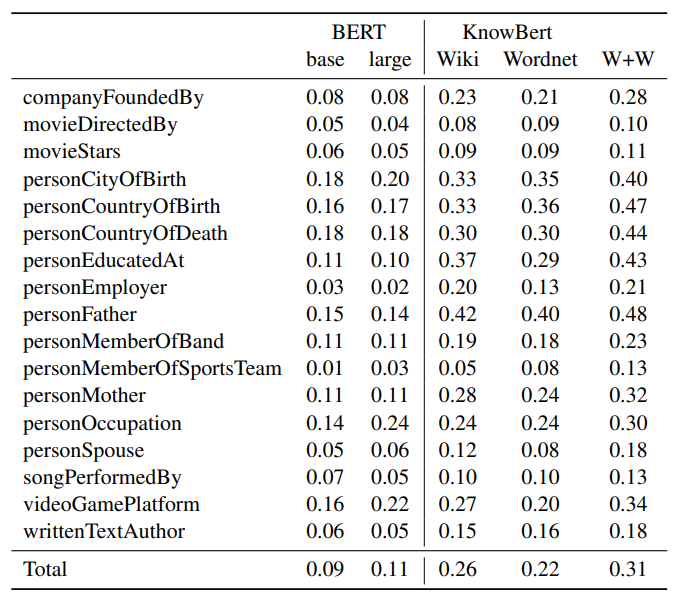
\includegraphics[height=0.8\textheight]{graphics/kb/wikidata_mrr.PNG}
    \end{figure}
    Courtesy of Peters et al. - we obtained similar results on all categories.
\end{frame}


\begin{frame}{The guts of KAR: Hamlet}
    \KARPLOT{3}
\end{frame}
\begin{frame}{The guts of KAR: Hamlet (Entities)}
    \vspace{-0.1cm}
\begin{table}[t!]
\tiny
\centering
\begin{tabular}{|p{2.4cm}|p{2.8cm}c|p{2.8cm}c|}
\hline
\multirow{3}{*}{\textbf{Candidate Spans}} & \multicolumn{4}{c|}{\textsf{hamlet is a book that was written by william shakespeare . }} \\
& \multicolumn{2}{c}{Priors (top-2)} & \multicolumn{2}{c|}{Norm. EL Scores (top-2)} \\ \cline{2-5}
& \multicolumn{1}{c|}{\textsf{ent}} & $p(\mathsf{ent})$ & \multicolumn{1}{c|}{\textsf{ent}} & $\psi_{m,k}$ \\ \hline 
\multicolumn{5}{c}{\textbf{\textsf{Wiki}}}\\
\hline
\multirow{2}{*}{\textsf{hamlet}}& Hamlet & 0.46 & Hamlet (2009 TV film) & 0.03\\ 
& Hamlet (1948 film) & 0.04 & Hamlet, Indiana & 0.03\\\hline 
\multirow{2}{*}{\textsf{william shakespeare}}& William Shakespeare & 0.63 & William Shakespeare (American football) & 0.06\\ 
& William Shakespeare (American football) & 0.09 & To be, or not to be & 0.06\\\hline 
\multirow{2}{*}{\textsf{shakespeare}}& William Shakespeare & 0.57 & Geoffrey Shakespeare & 0.03\\ 
& Shakespeare's plays & 0.02 & Arthur Shakespeare & 0.03\\\hline 
\multicolumn{5}{c}{\textbf{\textsf{Wordnet}}}\\
\hline
\multirow{2}{*}{\textsf{hamlet}}& hamlet.n.01 & 0.50 & hamlet.n.01 & 1.00\\ 
& village.n.02 & 0.25 & village.n.02 & 0.00\\\hline 
\multirow{2}{*}{\textsf{is}}& be.v.01 & 0.64 & be.v.02 & 1.00\\ 
& be.v.02 & 0.18 & be.v.01 & 0.00\\\hline 
\multirow{2}{*}{\textsf{a}}& angstrom.n.01 & 0.50 & a.n.07 & 0.99\\ 
& a.n.07 & 0.07 & angstrom.n.01 & 0.01\\\hline 
\multirow{2}{*}{\textsf{book}}& book.n.01 & 0.59 & book.n.01 & 1.00\\ 
& book.n.02 & 0.14 & script.n.01 & 0.00\\\hline 
\multirow{2}{*}{\textsf{was}}& be.v.01 & 0.64 & be.v.01 & 0.99\\ 
& be.v.02 & 0.18 & be.v.02 & 0.01\\\hline 
\multirow{2}{*}{\textsf{written}}& write.v.01 & 0.38 & write.v.01 & 1.00\\ 
& write.v.02 & 0.32 & spell.v.03 & 0.00\\\hline 
\multirow{2}{*}{\textsf{by}}& by.r.01 & 0.75 & by.r.01 & 1.00\\ 
& aside.r.06 & 0.25 & aside.r.06 & 0.00\\\hline 
\multirow{2}{*}{\textsf{william shakespeare}}& shakespeare.n.01 & 1.00 & shakespeare.n.01 & 1.00\\ 
& N/A & 0.00 & N/A & 0.00\\\hline 
\end{tabular}
\end{table}
\end{frame}

% t-SNE 
\begin{frame}{Contextual Word Embeddings: t-SNE - from overview to sampled few}
    \begin{figure}
        \centering
        \includegraphics[height=0.15\textheight]{graphics/contextual_embeddings/new/tSNE_9512_1_2_baseline_testNoneNone.eps}
    \end{figure}
    \begin{figure}
        \centering
        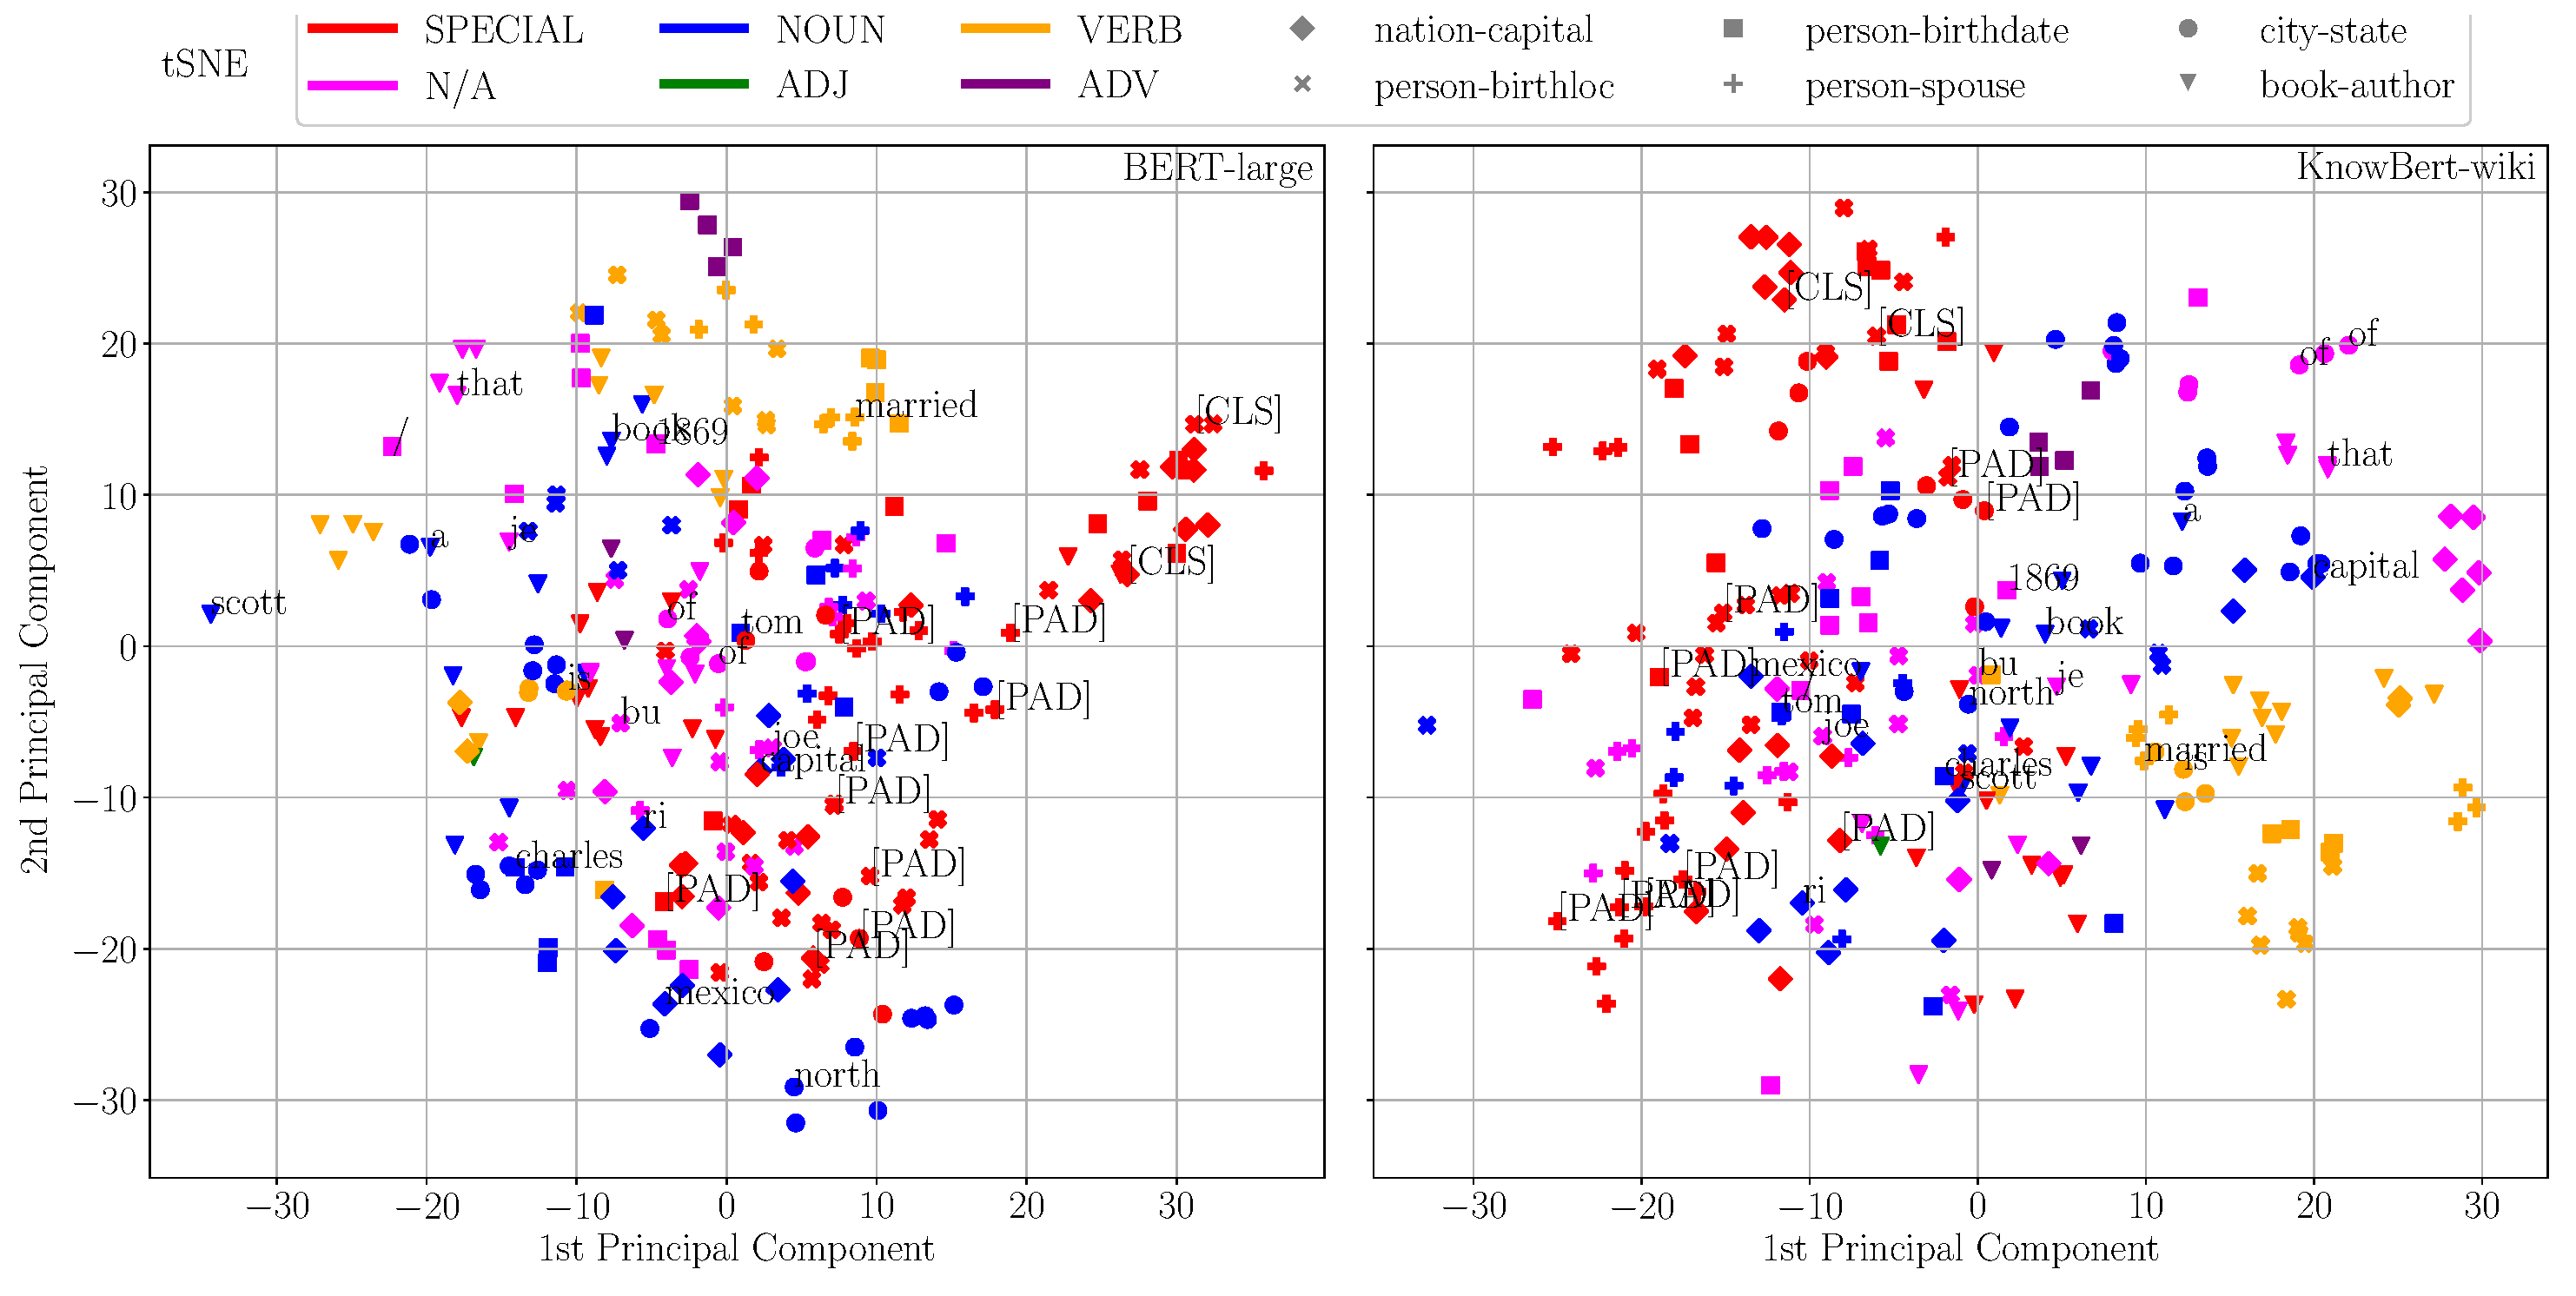
\includegraphics[height=0.78\textheight]{graphics/contextual_embeddings/new/tSNE_250_1_2_baseline_test_annotatedNone.eps}
    \end{figure}
\end{frame}

\begin{frame}{Contextual Word Embeddings: t-SNE - from overview to sampled few}
    \begin{columns}
        \begin{column}{0.5\textwidth}
        \textbf{KnowBERT-wordnet}
            \begin{figure}
                \centering
                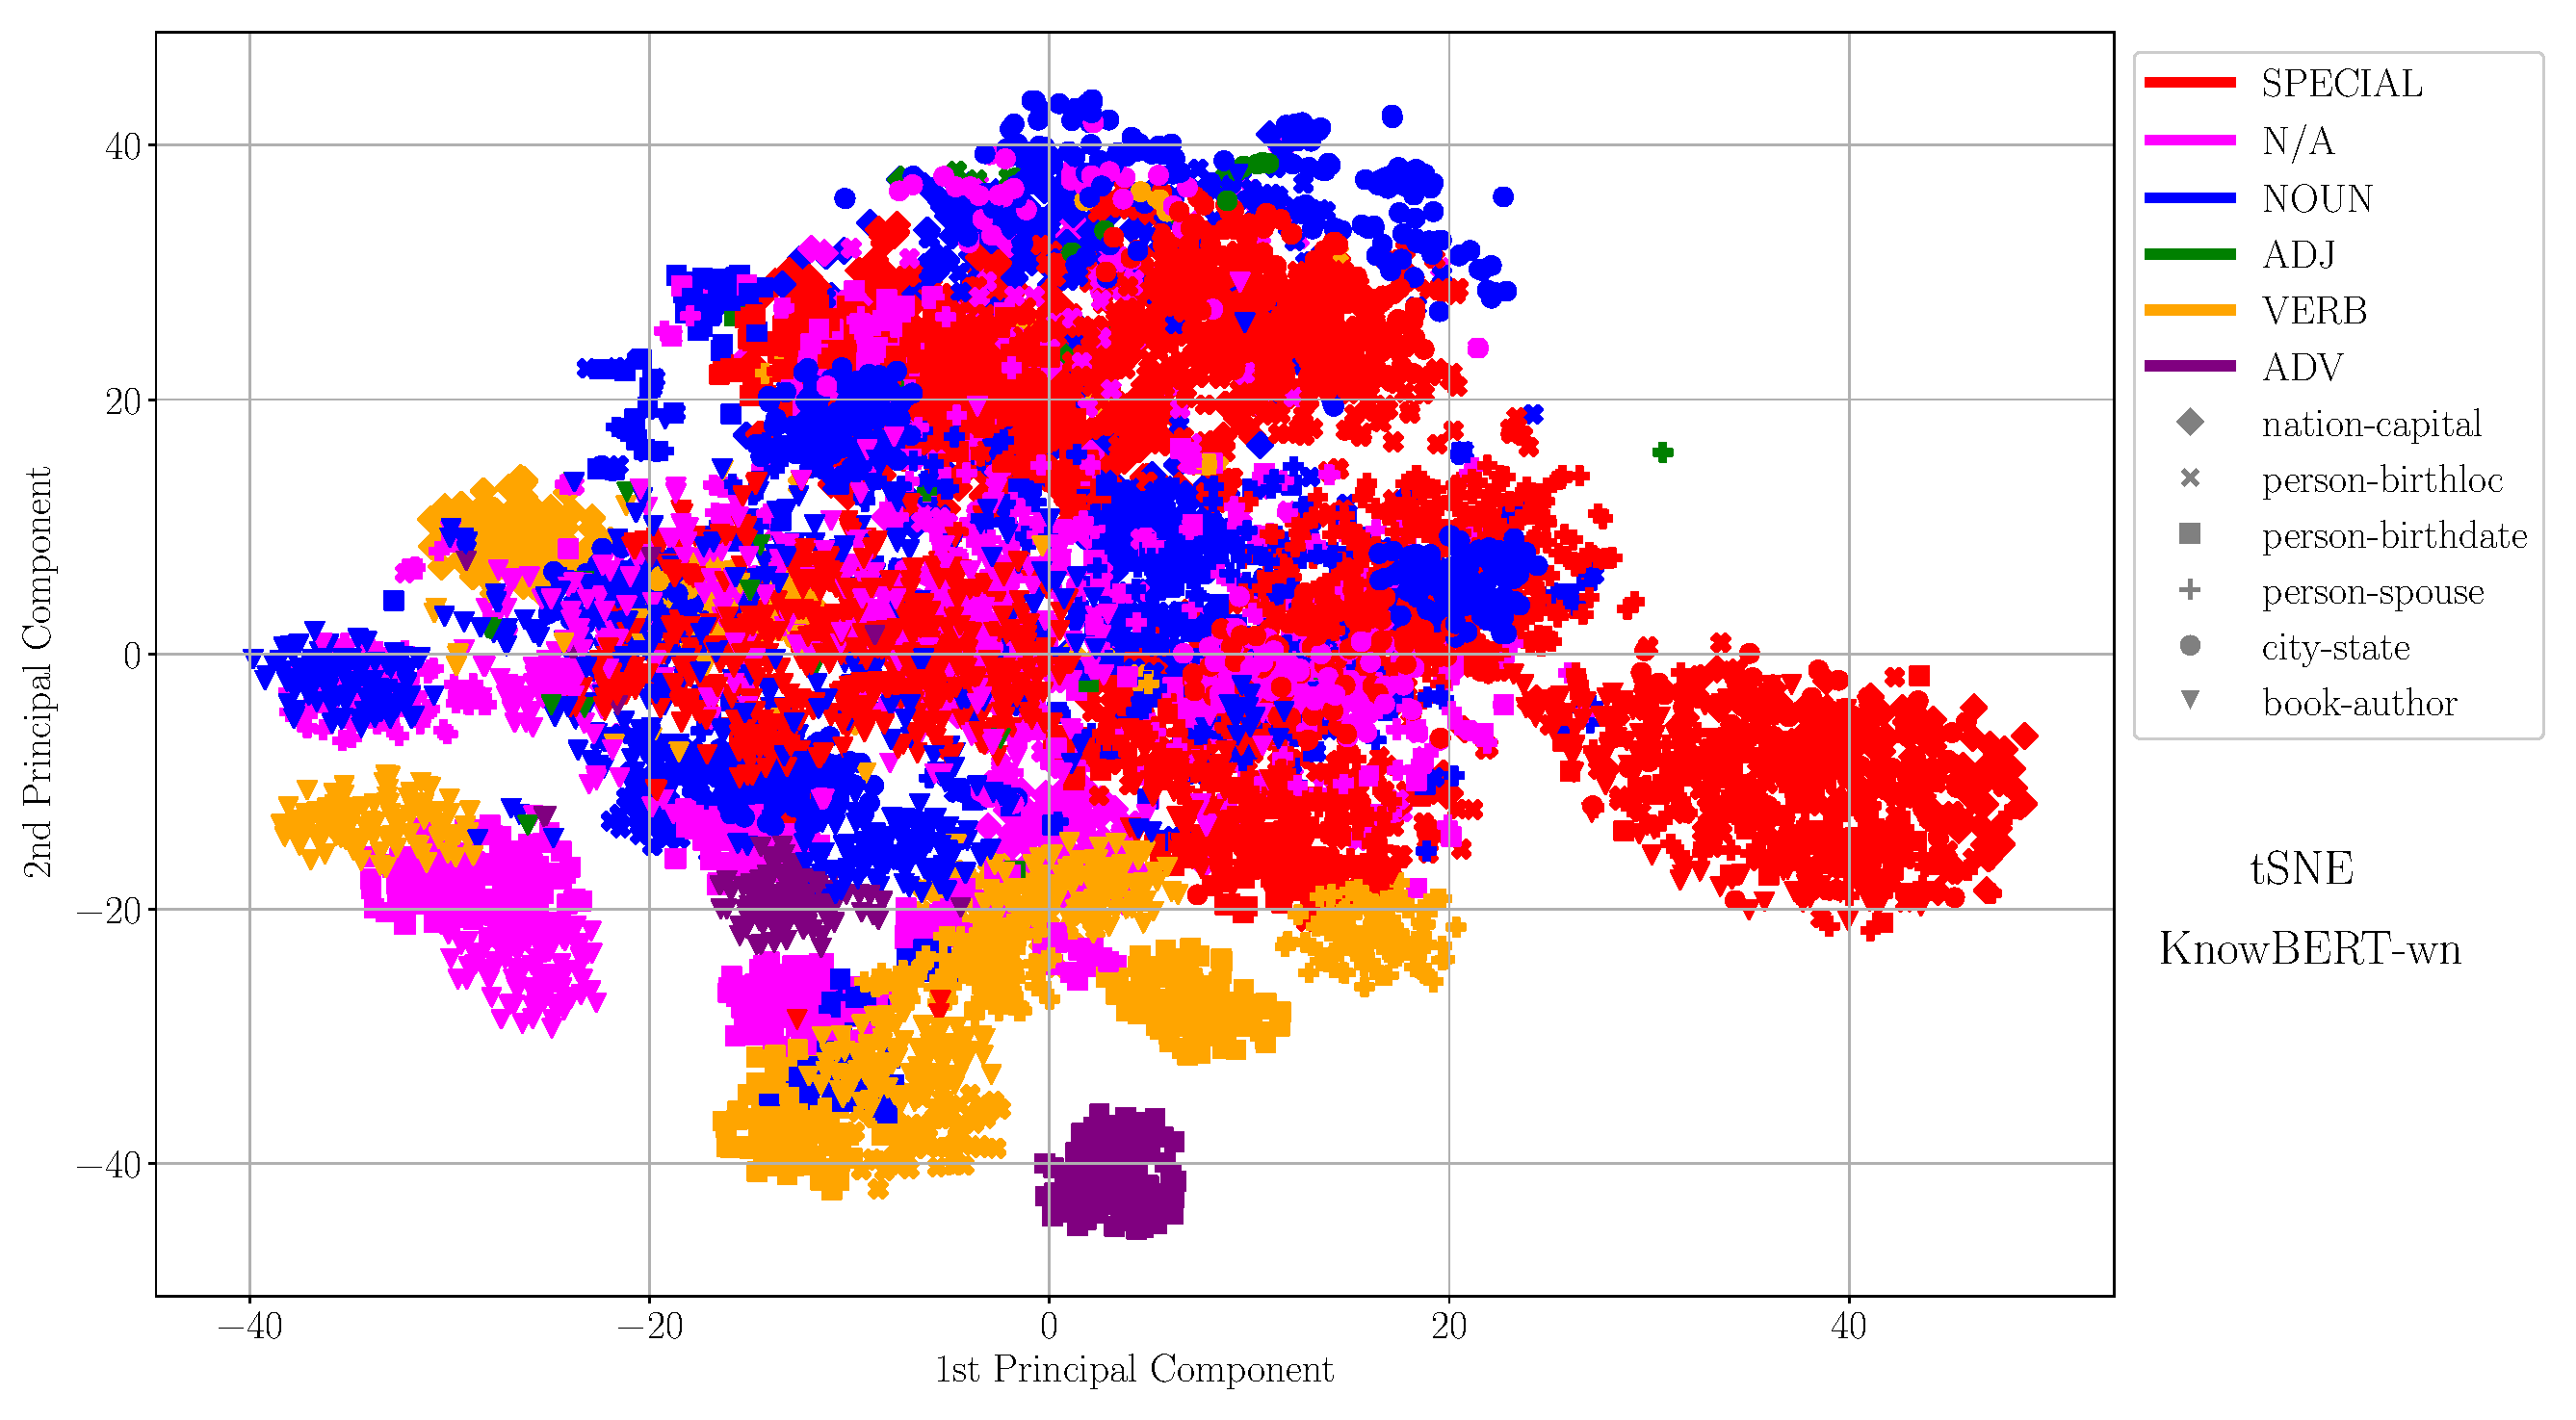
\includegraphics[height=0.15\textheight]{graphics/contextual_embeddings/tSNE_9512_1_2_knowbert_wordnetNone_title.eps}
            \end{figure}
            \begin{figure}
                \centering
                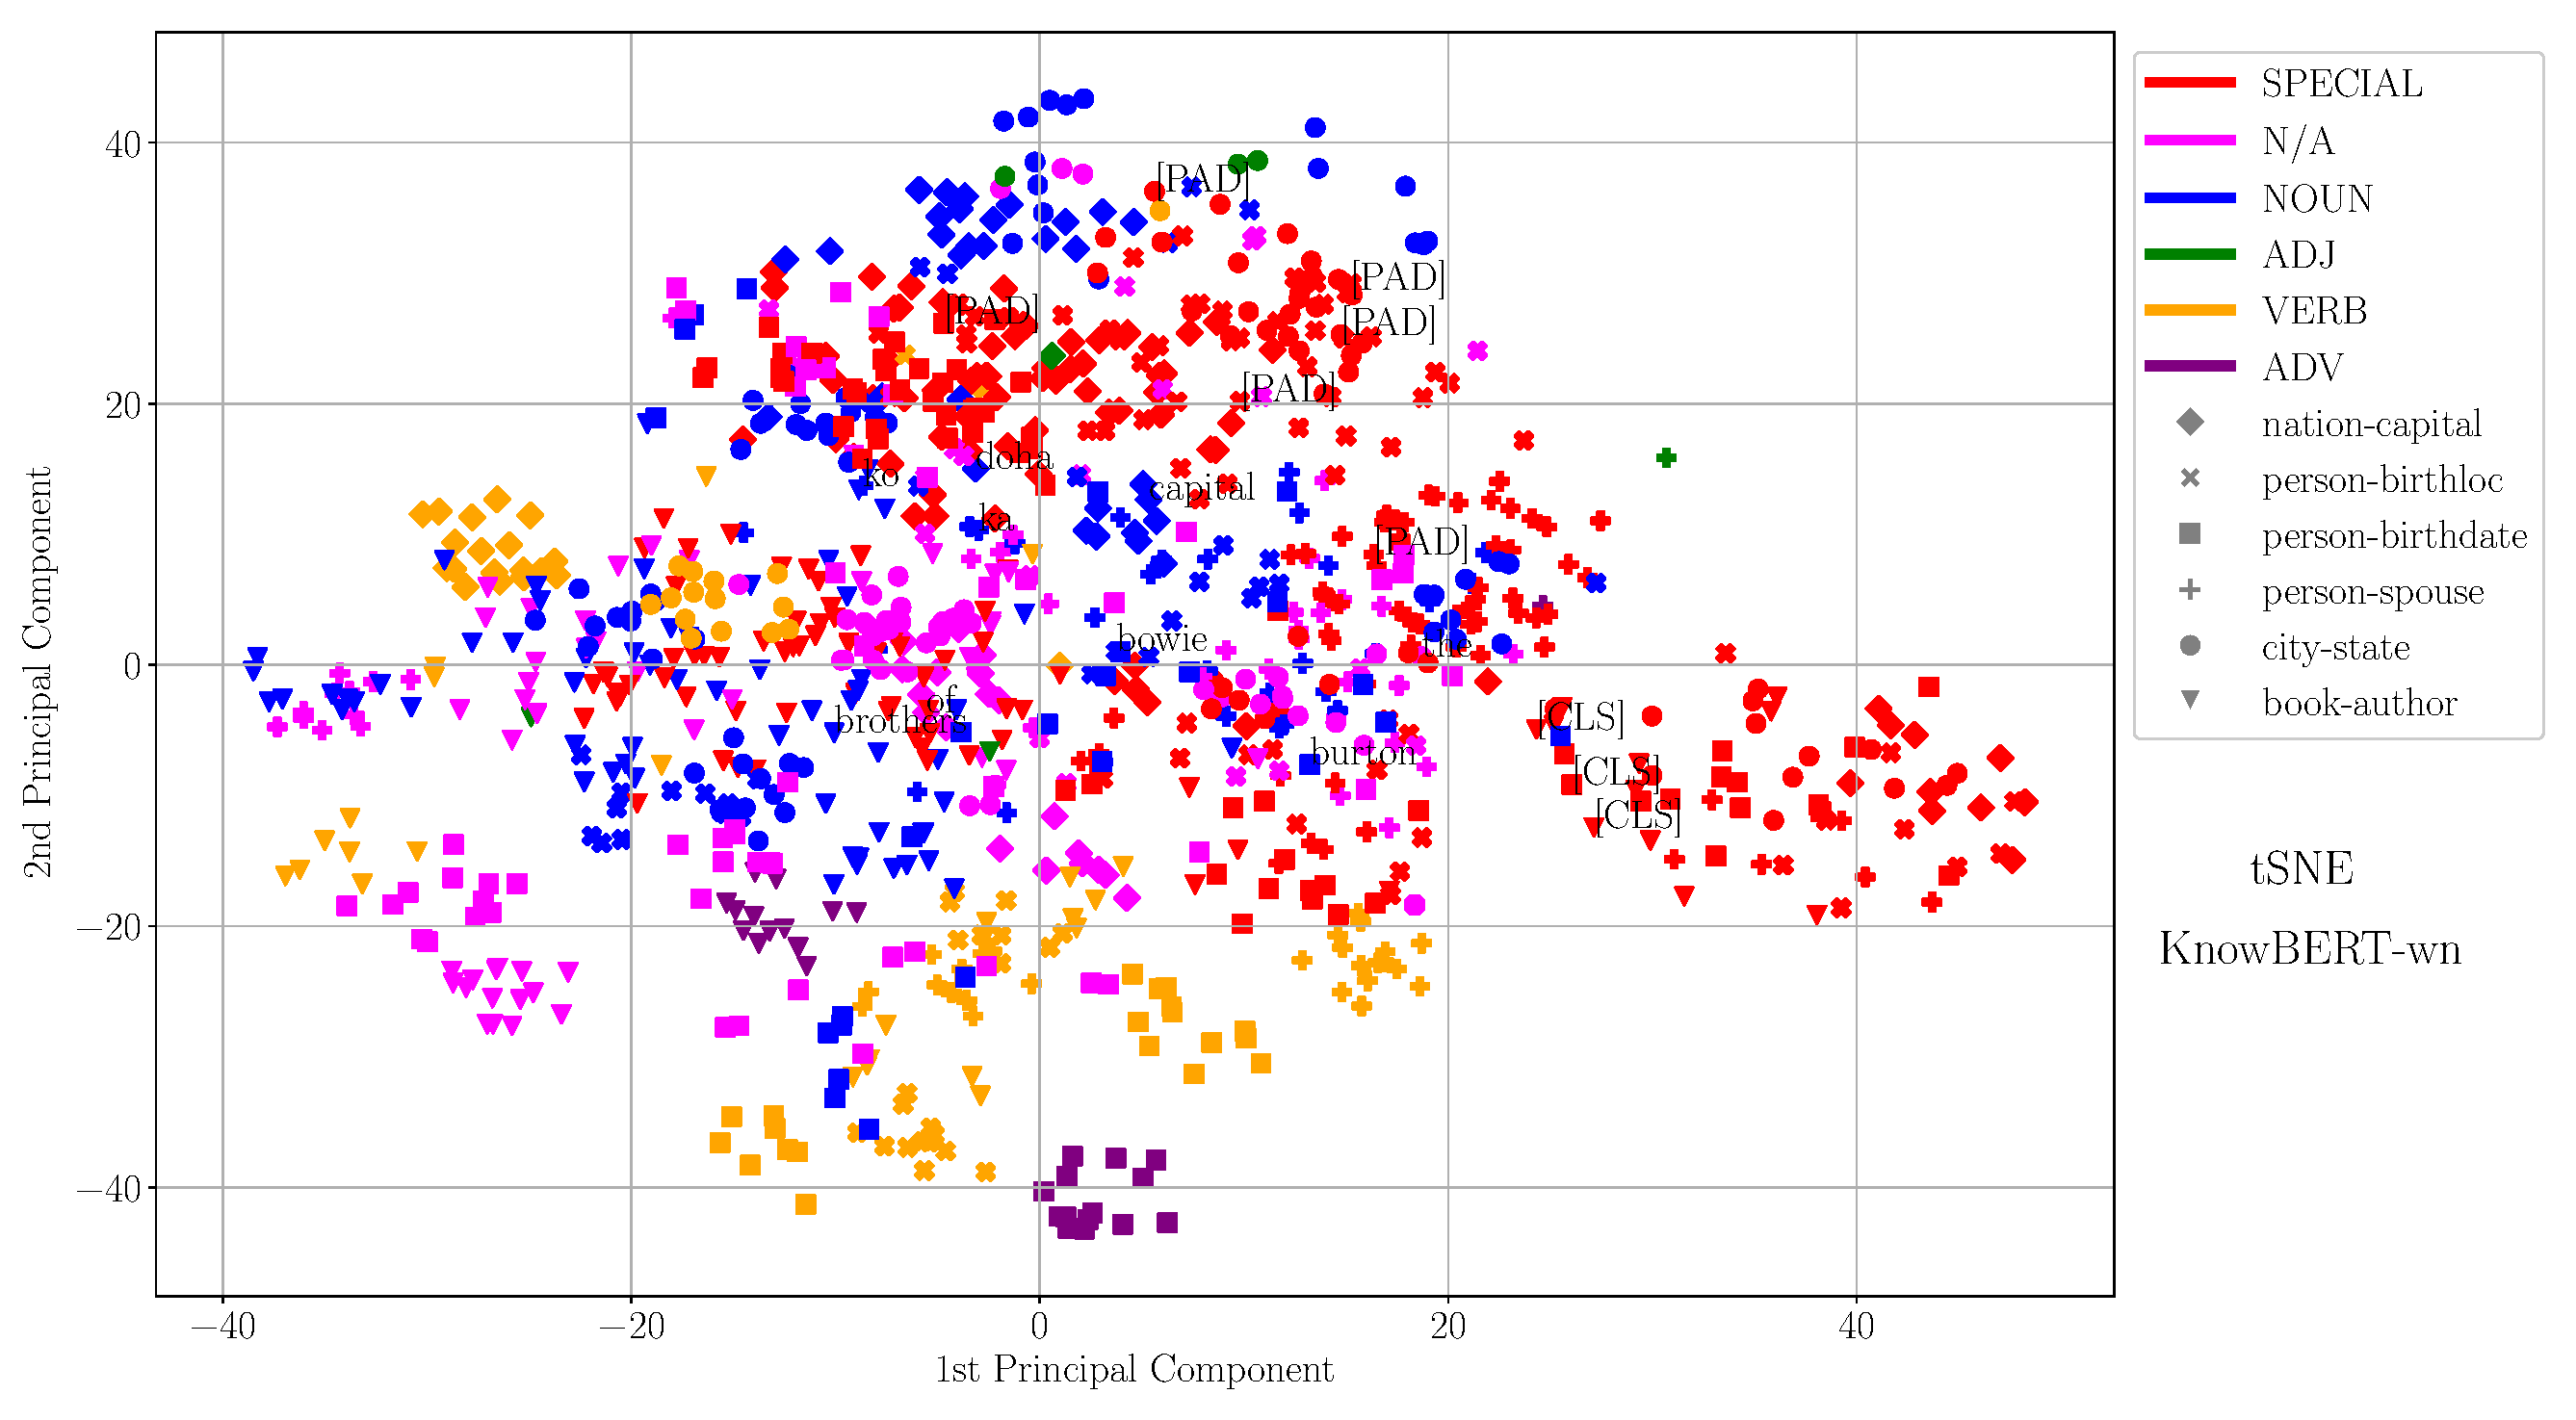
\includegraphics[height=0.55\textheight]{graphics/contextual_embeddings/tSNE_1024_1_2_knowbert_wordnet_annotated_title.eps}
            \end{figure}
        \end{column}
        \begin{column}{0.5\textwidth}
        \textbf{KnowBERT-W+W}
            \begin{figure}
                \centering
                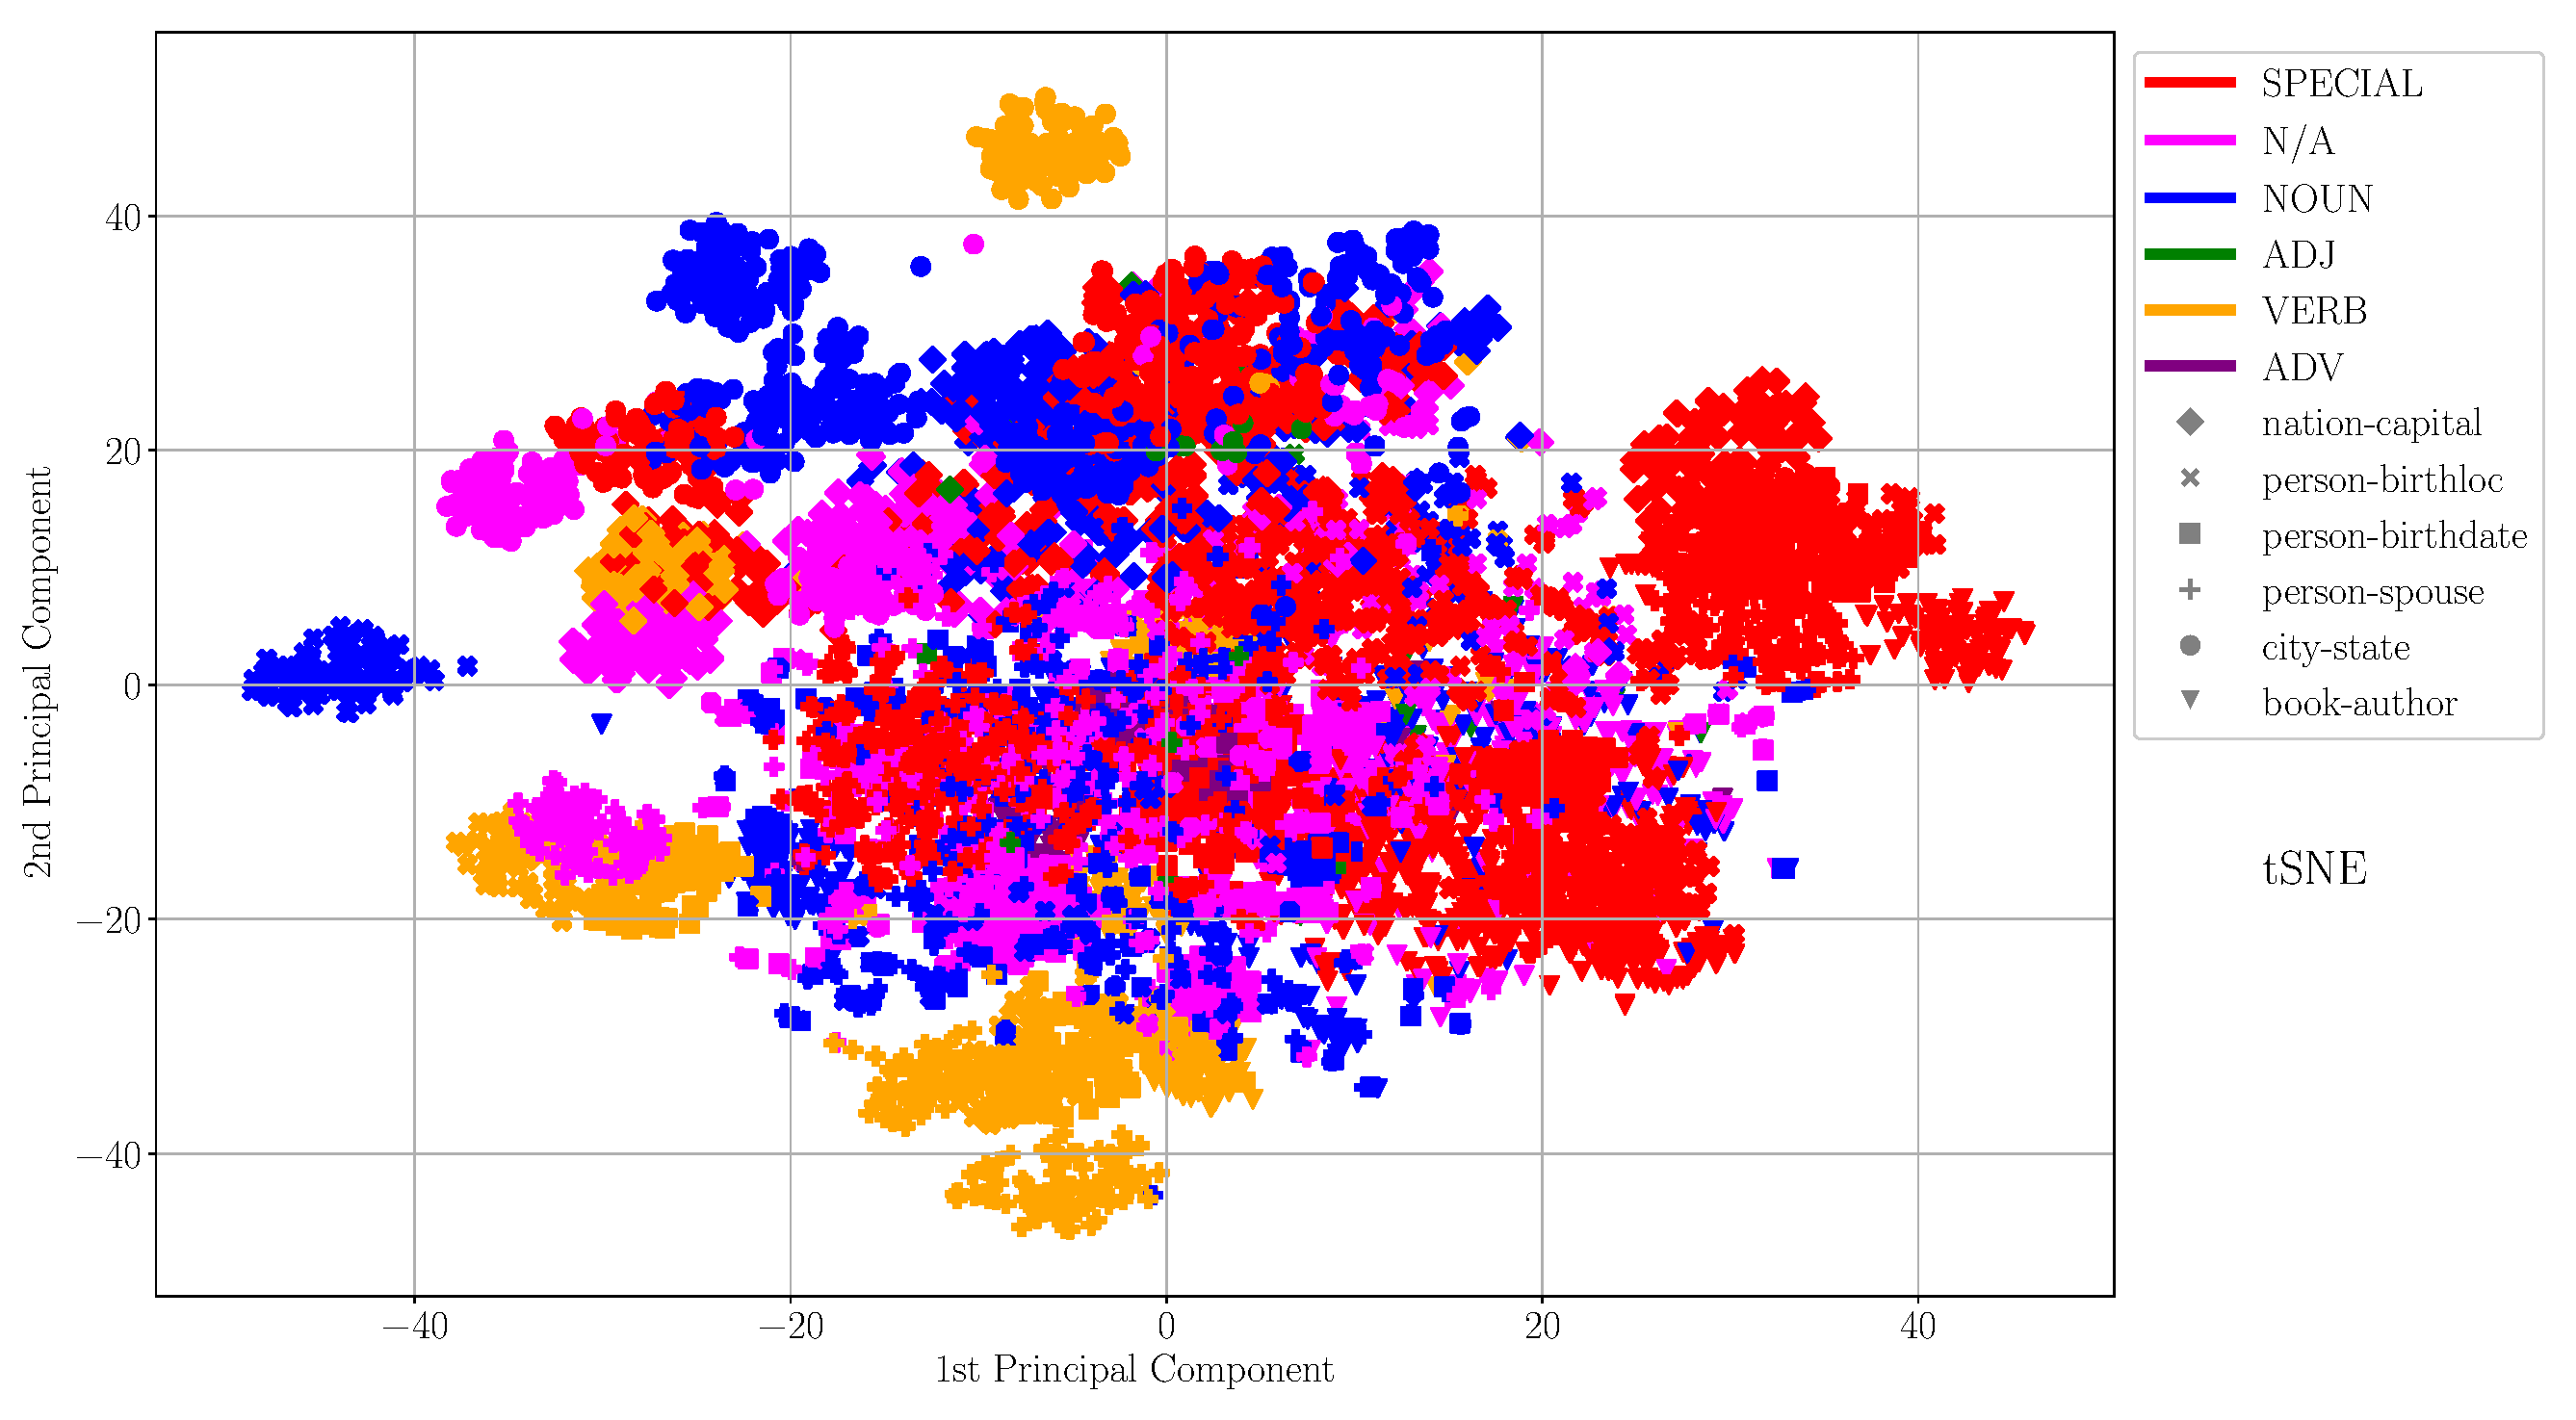
\includegraphics[height=0.15\textheight]{graphics/contextual_embeddings/tSNE_9512_1_2_knowbert_wiki_wordnetNone_title_USE.eps}
            \end{figure}
            \begin{figure}
                \centering
                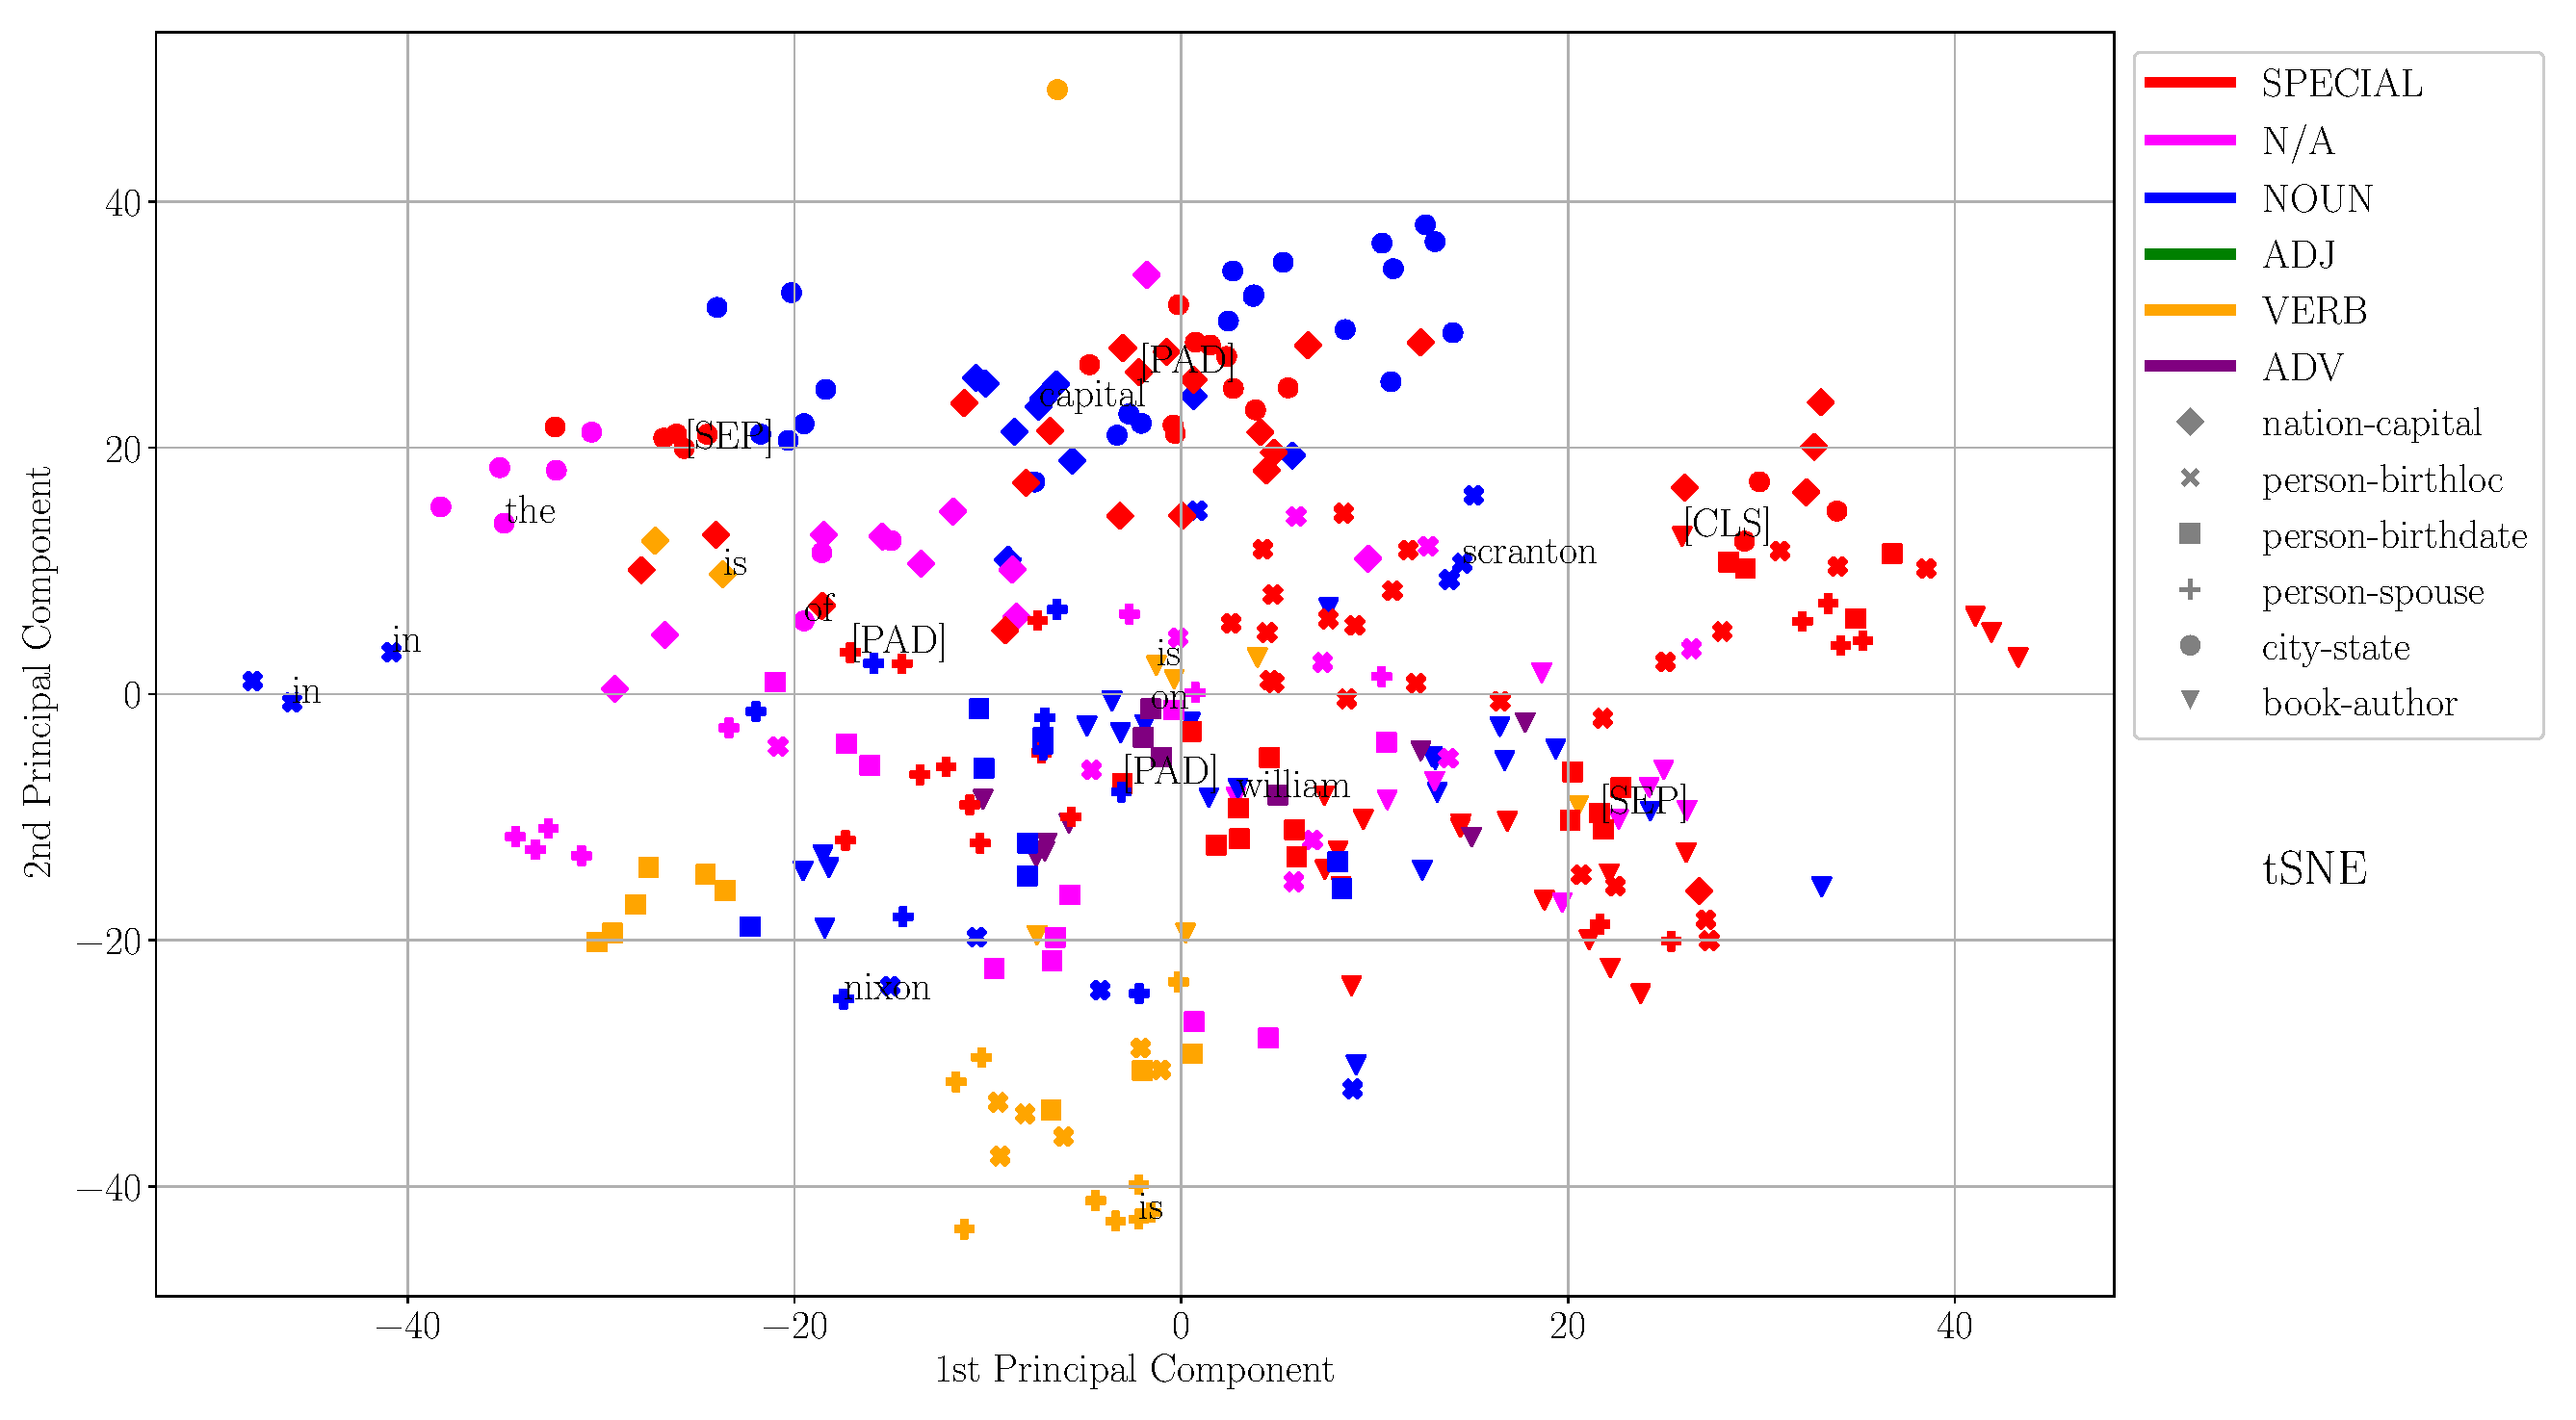
\includegraphics[height=0.55\textheight]{graphics/contextual_embeddings/tSNE_300_1_2_knowbert_wiki_wordnet_annotated_title.eps}
            \end{figure}
        \end{column}
    \end{columns}
\end{frame}


